\ifdefined\ReaderVersion
  \documentclass[pdflatex,sn-vancouver-num,iicol]{sn-jnl}
\else
  \documentclass[pdflatex,sn-vancouver-num]{sn-jnl}
\fi

\usepackage{amsmath,amssymb,mathtools}
\usepackage{array,booktabs,multirow,tabularx}
\usepackage{graphicx,microtype,balance}
\usepackage{tikz,pgfplots}
\usepgfplotslibrary{groupplots}
\pgfplotsset{compat=1.18}
\newcommand{\KL}{\operatorname{KL}}
\usepackage{needspace}
\usepackage{url}
\ifdefined\ReaderVersion\else
  \usepackage[switch]{lineno}
  \usepackage{setspace}
\fi
\graphicspath{{figures/}}
\hypersetup{
  pdftitle={Assay resolution governs the transfer of molecular dependence},
  pdfauthor={Anonymous Authors}
}
% Machine-checked values from versioned result artifacts.
\newcommand{\SimReps}{128}
\newcommand{\SimHetSameHier}{0.01493}
\newcommand{\SimHetSameCommon}{0.01521}
\newcommand{\SimHetSameCommonReduction}{1.85\%}
\newcommand{\SimHetSameCommonReductionLo}{1.52\%}
\newcommand{\SimHetSameCommonReductionHi}{2.18\%}
\newcommand{\SimHetShiftHier}{0.01159}
\newcommand{\SimHetShiftCommon}{0.01171}
\newcommand{\SimHetShiftResidual}{0.03359}
\newcommand{\SimHetShiftResidualReduction}{65.49\%}
\newcommand{\SimHetShiftResidualReductionLo}{63.02\%}
\newcommand{\SimHetShiftResidualReductionHi}{67.72\%}
\newcommand{\SimHomSameHier}{0.008752}
\newcommand{\SimHomSameCommon}{0.008660}
\newcommand{\SimHomSameHierPenalty}{1.06\%}
\newcommand{\SimHomShiftHier}{0.008674}
\newcommand{\SimHomShiftCommon}{0.008640}
\newcommand{\SimHomShiftResidual}{0.02943}
\newcommand{\SimHomShiftResidualReduction}{70.52\%}
\newcommand{\SimHomShiftResidualReductionLo}{69.21\%}
\newcommand{\SimHomShiftResidualReductionHi}{71.74\%}
\newcommand{\RiskStressConditions}{48}
\newcommand{\RiskStressEnvelopePass}{48/48}
\newcommand{\RiskStressCoverage}{48/48}
\newcommand{\RiskStressIntegralError}{1.91\times10^{-14}}
\newcommand{\RiskStressMaxZ}{1.833}
\newcommand{\PSciN}{85}
\newcommand{\PSciR}{0.525}
\newcommand{\PSciRLo}{0.483}
\newcommand{\PSciRHi}{0.566}
\newcommand{\PSciRMSE}{0.844}
\newcommand{\PSciRMSELo}{0.819}
\newcommand{\PSciRMSEHi}{0.868}
\newcommand{\PSciDirectR}{0.429}
\newcommand{\PSciDestroyedR}{0.074}
\newcommand{\PSciFourStateR}{0.640}
\newcommand{\PSciNeighbor}{0.064}
\newcommand{\PSciNeighborLo}{0.050}
\newcommand{\PSciNeighborHi}{0.079}
\newcommand{\PSciDestroyedNeighbor}{0.051}
\newcommand{\PSciDestroyedNeighborLo}{0.041}
\newcommand{\PSciDestroyedNeighborHi}{0.063}
\newcommand{\PSciNeighborDiff}{0.013}
\newcommand{\PSciNeighborDiffLo}{-0.003}
\newcommand{\PSciNeighborDiffHi}{0.030}
\newcommand{\PSciNeighborP}{0.283}
\newcommand{\FrangiehN}{179}
\newcommand{\FrangiehR}{0.040}
\newcommand{\FrangiehRLo}{0.013}
\newcommand{\FrangiehRHi}{0.066}
\newcommand{\FrangiehRMSE}{1.009}
\newcommand{\PapalexiN}{24}
\newcommand{\PapalexiR}{-0.025}
\newcommand{\PapalexiRLo}{-0.150}
\newcommand{\PapalexiRHi}{0.096}
\newcommand{\PapalexiRMSE}{1.037}
\newcommand{\MultiN}{35}
\newcommand{\MultiR}{-0.224}
\newcommand{\MultiRLo}{-0.330}
\newcommand{\MultiRHi}{-0.124}
\newcommand{\MultiRMSE}{1.047}
\newcommand{\PerturbFateN}{49}
\newcommand{\PerturbFateR}{-0.092}
\newcommand{\PerturbFateRLo}{-0.152}
\newcommand{\PerturbFateRHi}{-0.035}
\newcommand{\PerturbFateRMSE}{1.023}
\newcommand{\ReSisArmP}{1/65}
\newcommand{\ReSisArmQ}{0.015}
\newcommand{\ReSisNKCos}{0.952}
\newcommand{\ReSisNKLo}{-0.801}
\newcommand{\ReSisNKHi}{0.968}
\newcommand{\ArceN}{28}
\newcommand{\ArceR}{0.412}
\newcommand{\ArceRLo}{0.331}
\newcommand{\ArceRHi}{0.494}
\newcommand{\ArceRMSE}{1.093}
\newcommand{\ArceRMSELo}{1.012}
\newcommand{\ArceRMSEHi}{1.185}
\newcommand{\ArceDecision}{refuse}
\newcommand{\StressNull}{3.0\%}
\newcommand{\StressPower}{96.5\%}
\newcommand{\StressHeavyNull}{5.5\%}
\newcommand{\StressGuidePower}{95.5\%}
\newcommand{\StressObsPower}{90.5\%}
\newcommand{\StephDevN}{36}
\newcommand{\StephHeldN}{56}
\newcommand{\StephPrimaryLoss}{0.01220}
\newcommand{\StephResidualLoss}{0.01478}
\newcommand{\StephResidualReduction}{17.46\%}
\newcommand{\StephResidualCILo}{-0.00413}
\newcommand{\StephResidualCIHi}{-0.00080}
\newcommand{\StephResidualFav}{50/56}
\newcommand{\StephSignP}{5.09\times10^{-10}}
\newcommand{\StephDestroyedLoss}{0.02274}
\newcommand{\StephDestroyedReduction}{46.36\%}
\newcommand{\StephDestroyedCILo}{-0.01323}
\newcommand{\StephDestroyedCIHi}{-0.00749}
\newcommand{\StephDestroyedFav}{51/56}
\newcommand{\StephRepeatedDestroyedN}{29}
\newcommand{\StephRepeatedDestroyedReduction}{47.30\%}
\newcommand{\StephRepeatedDestroyedReductionLo}{37.56\%}
\newcommand{\StephRepeatedDestroyedReductionHi}{54.59\%}
\newcommand{\StephRepeatedDestroyedDiffLo}{-0.01367}
\newcommand{\StephRepeatedDestroyedDiffHi}{-0.00795}
\newcommand{\StephRepeatedDestroyedFav}{51/56}
\newcommand{\StephRepeatedDestroyedP}{5.85\times10^{-11}}
\newcommand{\StephTLineageReduction}{-3.41\%}
\newcommand{\StephBLineageReduction}{-0.78\%}
\newcommand{\StephMyeloidReduction}{15.51\%}
\newcommand{\StephMyeloidReductionLo}{5.51\%}
\newcommand{\StephMyeloidReductionHi}{24.61\%}
\newcommand{\StephMyeloidFav}{21/46}
\newcommand{\StephMyeloidSignP}{0.769}
\newcommand{\StephCommonExactLoss}{0.01300}
\newcommand{\StephCommonExactReduction}{6.18\%}
\newcommand{\StephCommonExactReductionLo}{3.84\%}
\newcommand{\StephCommonExactReductionHi}{8.47\%}
\newcommand{\StephCommonExactCILo}{-0.00121}
\newcommand{\StephCommonExactCIHi}{-0.00046}
\newcommand{\StephCommonExactFav}{46/56}
\newcommand{\StephCommonExactSignP}{6.23\times10^{-7}}
\newcommand{\StephPooledPoissonLoss}{0.01263}
\newcommand{\StephPooledPoissonReduction}{3.39\%}
\newcommand{\StephPooledPoissonReductionLo}{1.42\%}
\newcommand{\StephPooledPoissonReductionHi}{5.37\%}
\newcommand{\StephPooledPoissonCILo}{-0.00075}
\newcommand{\StephPooledPoissonCIHi}{-0.00017}
\newcommand{\StephPooledPoissonFav}{38/56}
\newcommand{\StephPooledPoissonSignP}{0.00523}
\newcommand{\GSEDevN}{15}
\newcommand{\GSEHeldN}{9}
\newcommand{\GSEPrimaryLoss}{0.00851}
\newcommand{\GSEResidualLoss}{0.01413}
\newcommand{\GSEResidualReduction}{39.81\%}
\newcommand{\GSEResidualCILo}{-0.00710}
\newcommand{\GSEResidualCIHi}{-0.00423}
\newcommand{\GSEResidualFav}{9/9}
\newcommand{\GSESignP}{0.00195}
\newcommand{\GSEDestroyedLoss}{0.04029}
\newcommand{\GSEDestroyedReduction}{78.89\%}
\newcommand{\GSEDestroyedCILo}{-0.03567}
\newcommand{\GSEDestroyedCIHi}{-0.02816}
\newcommand{\GSEDestroyedFav}{9/9}
\newcommand{\GSECommonExactLoss}{0.00832}
\newcommand{\GSECommonExactRelative}{-2.20\%}
\newcommand{\GSECommonExactAdvantage}{2.20\%}
\newcommand{\GSECommonExactRelativeLo}{-3.03\%}
\newcommand{\GSECommonExactRelativeHi}{-1.34\%}
\newcommand{\GSECommonExactCILo}{0.00010}
\newcommand{\GSECommonExactCIHi}{0.00028}
\newcommand{\GSECommonExactFav}{0/9}
\newcommand{\GSECommonExactSignP}{1.000}
\newcommand{\GSEPooledPoissonLoss}{0.00996}
\newcommand{\GSEPooledPoissonReduction}{14.58\%}
\newcommand{\GSEPooledPoissonReductionLo}{11.94\%}
\newcommand{\GSEPooledPoissonReductionHi}{17.16\%}
\newcommand{\GSEPooledPoissonCILo}{-0.00181}
\newcommand{\GSEPooledPoissonCIHi}{-0.00115}
\newcommand{\GSEPooledPoissonFav}{9/9}
\newcommand{\GSEPooledPoissonSignP}{0.00195}
\newcommand{\GSEStandardPoissonLoss}{0.00998}
\newcommand{\GSEStandardPoissonReduction}{14.79\%}
\newcommand{\GSEStandardPoissonReductionLo}{12.18\%}
\newcommand{\GSEStandardPoissonReductionHi}{17.37\%}
\newcommand{\GSEStandardPoissonCILo}{-0.00184}
\newcommand{\GSEStandardPoissonCIHi}{-0.00117}
\newcommand{\GSEStandardPoissonFav}{9/9}
\newcommand{\GSEStandardPoissonSignP}{0.00195}
\newcommand{\CombatPrimaryLoss}{0.01156}
\newcommand{\CombatResidualLoss}{0.01561}
\newcommand{\CombatReduction}{25.94\%}
\newcommand{\CombatCILo}{-0.00597}
\newcommand{\CombatCIHi}{-0.00225}
\newcommand{\CombatFav}{17/24}
\newcommand{\BMMCPrimaryLoss}{0.01085}
\newcommand{\BMMCResidualLoss}{0.01315}
\newcommand{\BMMCReduction}{17.47\%}
\newcommand{\BMMCCILo}{-0.00504}
\newcommand{\BMMCCIHi}{-0.00038}
\newcommand{\BMMCFav}{4/4}
\newcommand{\GSEThreeOneFourPilotN}{20}
\newcommand{\GSEThreeOneFourPrimaryLoss}{0.001927}
\newcommand{\GSEThreeOneFourResidualLoss}{0.001936}
\newcommand{\GSEThreeOneFourResidualReduction}{0.49\%}
\newcommand{\GSEThreeOneFourResidualCILo}{-0.0000182}
\newcommand{\GSEThreeOneFourResidualCIHi}{-0.0000011}
\newcommand{\GSEThreeOneFourResidualFav}{13/20}
\newcommand{\GSEThreeOneFourDestroyedLoss}{0.001936}
\newcommand{\GSEThreeOneFourDestroyedReduction}{0.45\%}
\newcommand{\GSEThreeOneFourDestroyedCILo}{-0.0000390}
\newcommand{\GSEThreeOneFourDestroyedCIHi}{0.0000223}
\newcommand{\GSEThreeOneFourDestroyedFav}{11/20}
\newcommand{\GSEThreeOneFourBroadReduction}{2.54\%}
\newcommand{\GSEThreeOneSevenCalibrationN}{7}
\newcommand{\GSEThreeOneSevenVisitN}{28}
\newcommand{\GSEThreeOneSevenPrimaryLoss}{0.006530}
\newcommand{\GSEThreeOneSevenPoissonLoss}{0.006609}
\newcommand{\GSEThreeOneSevenPoissonReduction}{1.19\%}
\newcommand{\GSEThreeOneSevenPoissonFav}{6/7}
\newcommand{\GSEThreeOneSevenTimeFav}{4/4}
\newcommand{\GSEThreeOneSevenDestroyedLoss}{0.007904}
\newcommand{\GSEThreeOneSevenDestroyedReduction}{17.39\%}
\newcommand{\GSEThreeOneSevenDestroyedFav}{7/7}


\newcolumntype{Y}{>{\raggedright\arraybackslash}X}

\begin{document}
\raggedbottom
\ifdefined\ReaderVersion\else
  \newgeometry{left=25mm,right=25mm,top=23mm,bottom=25mm}
  \doublespacing
  \linenumbers
\fi
\title[Assay resolution and dependence transfer]{Assay resolution governs the transfer of molecular dependence}
\author*[1]{\fnm{Anonymous} \sur{Authors}}
\affil*[1]{\orgdiv{Affiliations withheld in the blinded manuscript}}

\abstract{
\textbf{Background:} Separate molecular assays retain coexpression even when cross-assay cell pairing is unavailable. We ask which recipient measurements are needed to transfer RNA--protein dependence from a paired reference.

\textbf{Results:} For finite assay profiles and a fixed interaction, we derive the sharp range of binary associations compatible with specified unpaired summaries and its minimax predictor. We evaluate reconstruction retrospectively in 24 Cambridge donors, 56 Newcastle donors, and 15 patients with pediatric T-cell acute lymphoblastic leukemia (T-ALL). With all recipient preprocessing and prediction inputs restricted to 256 adaptation cells, retaining both assay-pattern distributions reduced deviance on 256 untouched cells by 16.6\%, 29.2\%, and 55.6\% relative to individual frequencies (paired recipient-bootstrap 95\% intervals, 13.0--20.3\%, 25.0--33.3\%, and 47.2--62.7\%). Both patterns also improved on protein patterns alone in every cohort. In a separate fixed-frequency comparison, covariances retained 91--97\% of the pattern-level gain and recipient-specific structure outperformed larger matched pools. A covariance response formula identified queries benefiting from this correction, improving prioritization over direct interaction strength in Newcastle and T-ALL.

\textbf{Conclusions:} Assay summaries determine both the identifiable range of molecular dependence and the information available for its prediction. Preserving recipient coexpression improves held-cell prediction without supplying scoring-cell frequencies or cross-assay pairings.
}
\keywords{single-cell multi-omics; molecular dependence; coarsening; statistical matching; optimal transport}
\maketitle

\section{Background}
Joint single-cell assays reveal how molecular measurements covary within cells.
When a new cohort supplies the assays separately, a paired reference can support
prediction of the missing joint distribution. The recipient still provides two
kinds of information: the frequency of each molecular state and the patterns
of states observed together within each assay. These are different constraints
on the cross-assay prediction.

Association models separate an interaction from its marginal distributions
and estimate it through conditional or density-ratio methods
\cite{sei,sei2026}. Inverse optimal transport learns an interaction from paired
observations \cite{li}, and CHAMPOLLION applies this approach to multi-omic
bridge integration \cite{champollion}. We ask how the resolution of recipient
observations changes the relationships that such a model can recover. A coarse
RNA--protein association can change when the frequencies of finer cellular
patterns change, even if the fine interaction is fixed. This connects
cross-cohort prediction to the noncollapsibility of marginal association
\cite{ghosh,bergsma2002}. Existing methods reconstruct a joint table from
specified marginals and interaction parameters \cite{hammond2024}. Here the
complete marginals can themselves be unknown: observed within-assay summaries
constrain them, leaving a set of possible coarse associations.

For finite assay supports and a specified interaction, we derive the sharp
range of binary associations compatible with unpaired summaries that determine
the query frequencies. The range gives a minimax prediction and quantifies
ambiguity remaining after those summaries are known exactly. It includes the
case in which every individual marker frequency is supplied; retaining only
the two queried frequencies gives a closed form.
We then test whether preserving within-assay structure improves prediction
on untouched recipient cells. Each comparison holds the source interaction,
cells, and estimated recipient marker frequencies fixed, separating the value
of retained information from differences between fitted estimators.
To identify which structure matters, we preserve recipient covariances with
pairwise maximum-entropy models \cite{schneidman}, then compare them with
models built from source donors or other recipients in the same cohort.
A response expansion explains how recipient coexpression changes a transferred
association and gives a query-ranking rule computable from unpaired assays.

\section{Methods}
\subsection{Reconstruction at the observed assay resolution}
Let $x$ and $y$ denote RNA and protein profiles on finite supports. A finite transferred interaction
$S(x,y)$ defines a family of recipient distributions
\begin{equation}
 q(x,y)=\exp\{S(x,y)+a(x)+b(y)\}.
 \label{eq:joint}
\end{equation}
The adjusting functions $a$ and $b$ enforce the observed recipient assay
distributions, including normalization. When both assay distributions are
known and strictly positive, they determine a unique reconstruction \cite{sei}. Molecular queries are
obtained by summing its probabilities over the corresponding profile states.

When only individual marker frequencies are retained, we instead fit the
exponential-family distribution whose adjusting functions are linear in the
marker indicators. The same interaction therefore supports several
reconstructions, depending on the recipient constraints. The means-only model
constrains marker frequencies but leaves within-assay dependence unconstrained.

\subsection{A sharp limit at the observed resolution}
Let the observed RNA and protein summaries be arbitrary finite collections of
within-assay means. Assume they define nonempty convex polytopes $\mathcal R$ and $\mathcal C$
of complete assay distributions consistent with those summaries. For each
$r\in\mathcal R$ and $c\in\mathcal C$, entropic reconstruction gives the unique
joint distribution $Q_S(r,c)$ with interaction $S$ and assay marginals $r,c$,
allowing zero-mass assay states (Additional file 1).
For a binary query $U=f(x)$ and $V=g(y)$, define
\begin{align*}
 \ell&=\min_{r\in\mathcal R,c\in\mathcal C}
       \Pr_{Q_S(r,c)}(U=1,V=1),\\
 h&=\max_{r\in\mathcal R,c\in\mathcal C}
       \Pr_{Q_S(r,c)}(U=1,V=1).
\end{align*}
If the summaries determine the query frequencies
$m_U=\Pr(U=1)$ and $m_V=\Pr(V=1)$, the set of query tables from these reconstructions is
exactly
\begin{equation}
 \left\{
 \begin{pmatrix}1-m_U-m_V+t&m_V-t\\m_U-t&t\end{pmatrix}:
 \ell\leq t\leq h
 \right\}.
 \label{eq:all-marker-interval}
\end{equation}
The result follows because $\mathcal R\times\mathcal C$ is compact and
connected and the matrix-scaled reconstruction is continuous. It is the sharp
identified set when all individual marker frequencies are supplied: take the
defining means of $\mathcal R$ and $\mathcal C$ to be the frequencies of all
markers. Complete assay-profile histograms collapse both polytopes to points.
These are the constraints used by the means-only and full-pattern
reconstructions. Additional file 1 gives the formal result and proof.

The means-only exponential-family fit selects one member of this set by
information projection. The interval records what the supplied frequencies
identify without that additional selection.

Write $P(t)$ for the table in Eq.~\eqref{eq:all-marker-interval}. The unique
minimax table $P_*$ equalizes the forward Kullback--Leibler (KL)
loss from the endpoint tables $P(\ell)$ and $P(h)$:
$\KL(P(\ell)\Vert P_*)=\KL(P(h)\Vert P_*)$. Within this fixed-interaction
family with exact population summaries, no predictor has smaller worst-case forward
KL loss. Computing
$\ell$ and $h$ requires global optimization over the marginal polytopes;
these outer problems need not be convex. The interval is an analytic
characterization, not a general efficient endpoint algorithm.
\ifdefined\ReaderVersion\needspace{5\baselineskip}\fi
Writing $\mathcal H(P)=-\sum P\log P$, its log odds are
\begin{equation}
 \theta_*=\frac{\mathcal H(P(\ell))-\mathcal H(P(h))}{h-\ell}
 \quad(\ell<h).
 \label{eq:minimax}
\end{equation}

When the recipient retains only the two queried frequencies, the endpoints
have a closed form. For a fine rectangle with
$f(x_0)=g(y_0)=0$ and $f(x_1)=g(y_1)=1$, define its interaction contrast
\begin{equation}
 d=S(x_0,y_0)+S(x_1,y_1)-S(x_0,y_1)-S(x_1,y_0).
 \label{eq:contrast}
\end{equation}
Let $L$ and $H$ be the smallest and largest such contrasts. The compatible
coarse log odds fill $[L,H]$ in closure, so $\ell$ and $h$ are the cell
probabilities with margins $m_U,m_V$ and log odds $L,H$. The information-radius
argument uses classical minimax KL geometry \cite{vanerven}; our
resolution-specific result is the exact interval induced by the observed
within-assay constraints.

To see the interval directly, sum the fine-table identity
$q(x_0,y_0)q(x_1,y_1)=e^d q(x_0,y_1)q(x_1,y_0)$ over all rectangles.
The coarse odds ratio is a positively weighted average of $e^d$, placing its
log in $[L,H]$. Concentrating each assay margin on an extremizing pair of
profiles attains either endpoint in closure. Continuity over the connected
set of compatible margins fills the interval between them.

\subsection{Individual frequencies can all agree}
The ambiguity also occurs when every marker's individual frequency is known.
Consider two binary RNA markers and one protein marker, coded as
$Z_1,Z_2,W\in\{-1,1\}$, each with mean zero. Fix the fine interaction to
$S=JZ_2W$, with $J\ne0$. Let the recipient RNA distribution have correlation
$\rho=\mathbb E(Z_1Z_2)$. Reconstruction gives
\begin{equation}
 \mathbb E(Z_1W)=\rho\tanh J.
 \label{eq:example}
\end{equation}
Changing $\rho$ from negative to positive reverses the queried RNA--protein
association without changing $J$ or any individual marker frequency. Separate
RNA profiles reveal $\rho$; their individual frequencies do not. As $\rho$
ranges over its compatible values, the all-marker interval for
$\Pr(Z_1=1,W=1)$ is
$[(1-|\tanh J|)/4,(1+|\tanh J|)/4]$. The example therefore gives a nondegenerate
instance of Eq.~\eqref{eq:all-marker-interval}, not a separate ambiguity claim.

\ifdefined\ReaderVersion\needspace{12\baselineskip}\fi
\subsection{How coexpression changes the prediction}
For fixed positive assay distributions on finite supports, scale a bilinear
interaction as $S_t(x,y)=t x^\top B y$, where $B$ is the source interaction
matrix and $t$ sets its strength. Let $\Sigma_x$ and $\Sigma_y$ be the two
within-assay covariance matrices. Near independence, the reconstructed
cross-assay covariance satisfies
\begin{equation}
 \operatorname{Cov}_{q_t}(X,Y)=t\Sigma_x B\Sigma_y+O(t^2).
 \label{eq:response}
\end{equation}
To first order, each predicted RNA--protein covariance sums source
interactions weighted by recipient covariances in both assays. A source
coefficient therefore need not equal the marginal association observed in a
new population. This is the multivariate counterpart of
Eq.~\eqref{eq:example}.

This local formula is the initial value of an exact finite-strength identity.
Let $s_t=\partial_t\log q_t(X,Y)$ be the score along the fixed-marginal
reconstruction, and write $\bar X=X-\mathbb E_rX$ and
$\bar Y=Y-\mathbb E_cY$. The marginal constraints give
$\mathbb E_{q_t}(s_t\mid X)=\mathbb E_{q_t}(s_t\mid Y)=0$, and hence
\begin{equation}
 \operatorname{Cov}_{q_1}(X,Y)
 =\int_0^1\mathbb E_{q_t}\{\bar X\bar Y^\top s_t\}\,dt.
 \label{eq:response-integral}
\end{equation}
At independence, $s_0=\bar X^\top B\bar Y$, which recovers
Eq.~\eqref{eq:response}.

The second-order term contracts two copies of $B$ with the third central
moments of each assay (Additional file 1). Thus preserving means and
covariances preserves the first-order prediction but does not determine the
prediction at the fitted interaction strength. The expansion specializes the dependence-model
score-projection identities of Sei and Yano \cite{sei}; it motivates a controlled test
of covariance against complete pattern information.

The response also predicts which queries are sensitive to replacing recipient
coexpression by pooled structure. For a binary query with nonconstant marker
frequencies, subtract the queried entries of $\Sigma_x B\Sigma_y$ for the
recipient and pool, square the difference, and divide by the product of the
two marker variances. This is the leading coefficient of twice the KL divergence
between their query distributions near independence
(Additional file 1). We test whether this score identifies relationships
whose empirical prediction improves with recipient-specific reconstruction.

In the fixed-frequency analysis, we evaluated the response rule along
$t\in\{0.05,0.10,0.25,0.50,0.75,1\}$. At each value, we exactly reconstructed
the recipient covariance model and the leave-one-recipient-out cohort-pool
model, then compared the response coefficient with twice the forward KL
divergence between their 81 query tables. We report pooled and within-recipient
Spearman correlations, top-27 overlap, and the ratio of exact discrepancy to
its quadratic approximation. Recipient-bootstrap intervals used 20,000 draws
with seed 906095.

\subsection{Data and recipient information}
The source comprised 12 Cambridge calibration donors from the Stephenson
CITE-seq (cellular indexing of transcriptomes and epitopes by sequencing)
study \cite{stephenson2021}. Recipients comprised the remaining 24
Cambridge donors, 56 Newcastle donors, and all 15 diagnosis patients in the
public pediatric T-ALL study, GSE248287 \cite{wiggers}, which sorted and remixed
immune and malignant cells before sequencing. The fixed panel was
CD4, CD7, CD14, CD19, CD33, CD38, CD44, CD47, and CD52 in both assays.
Each person contributed 512 cells selected deterministically without consulting
their molecular counts. The first 256 cells supplied adaptation profiles;
the remaining 256 supplied evaluation tables. Cross-assay correspondence in
the adaptation half was discarded, so reconstruction received two separate
assay distributions.

\subsection{Prediction from adaptation cells alone}
RNA states recorded detection. For each person and protein, the median count
among the 256 adaptation cells defined a threshold. Counts strictly above this
threshold were high; ties were low. The same threshold was applied to scoring
cells without using their values to define it.

We fitted the source interaction once on the 12 Cambridge source donors under
these state definitions, using pairing contrasts with penalty $10^{-4}$.
The contrasts compare observed cell pairs with within-donor swaps and remove
additive assay effects from the likelihood \cite{sei}. A product-Bernoulli
source prior with total pseudocount mass four smoothed each recipient
adaptation histogram. The resulting
histograms determined every recipient marginal constraint; no scoring-cell
frequencies or pairings entered prediction.

The four reconstructions retained individual frequencies, RNA patterns plus
protein frequencies, protein patterns plus RNA frequencies, or both pattern
distributions. All used the same interaction and the same estimated marker
frequencies. An independence control used the product of those frequencies.
Predictions were fixed before scoring the remaining 256 cells. Full patterns
were compared with individual frequencies, protein patterns, and independence
in each cohort, giving nine contrasts. Additional file 1 specifies the source
fit, smoothing, and numerical checks.

\subsection{Fixed-frequency decomposition of the information gain}
To isolate dependence prediction from errors in estimated marker frequencies,
we also analyzed the same recipients conditional on their scoring-cell
frequencies. This analysis used the original donor-wide protein states and
source fit described below. Its losses are reported separately because its
states and permitted information differ from adaptation-only prediction.

RNA states recorded detection. Protein states divided each person's 512 cells
into lower and upper rank halves, with deterministic hash-based tie breaking.
The first 256 cells supplied separate RNA and protein
pattern histograms. A source prior with total pseudocount mass four smoothed each histogram,
which was tilted to the individual marker frequencies of the remaining 256
cells. Cross-assay pairings in those remaining cells were used only for scoring.

We estimated $B$ in the binary interaction $S(x,y)=x^\top B y$ by pairing
contrasts, with penalty $10^{-4}$ selected on source donors. These contrasts
compare observed pairs with their within-donor swaps, removing additive assay
effects from the likelihood \cite{sei}. The same fitted $B$ was used in every arm without
refitting or recipient tuning.

The four arms retained individual frequencies alone, RNA patterns plus protein
frequencies, protein patterns plus RNA frequencies, or both pattern
distributions. Each arm used the exponential-family reconstruction satisfying
its specified constraints. Complete pattern constraints were fitted by matrix
scaling; individual frequency constraints were fitted by moment matching.

For the covariance intervention, we replaced each smoothed, tilted assay
distribution by the maximum-entropy distribution matching its first and second
marker moments. On a binary panel this distribution has unary and pairwise
log-linear terms \cite{schneidman}. Reconstruction used these replacement
marginals and the unchanged $B$. The intervention preserves measured
coexpression but replaces pattern structure not determined by those moments.

To test recipient specificity, we constructed two pooled controls from the
first 256 cells of either the 12 source donors or all other recipients in the
query person's cohort. The latter pool excluded the query person and contained
23 Cambridge donors, 55 Newcastle donors, or 14 T-ALL patients. Each contributor
added prior mass four, preserving the prior fraction. Pooled histograms
underwent the same tilting to recipient marker frequencies and maximum-entropy
replacement. The cohort control used other recipients' unpaired profiles;
neither control used their scoring-cell patterns.

For query prioritization, the response score used the recipient and cohort-pool
covariances. The comparator used the squared direct source coefficient
$B_{ij}^2$ multiplied by the two marker variances. Each rule ranked all 81 pairs
within each person, with zero assigned to constant-marker queries and ties
resolved by the fixed marker order. The top-third comparison and scores were fixed before calculating
pair-specific losses. We compared the mean deviance gain among the response
score's top 27 and bottom 27 pairs, then compared its top 27 with the
comparator's top 27. Both rules used the same recipient predictions; only the
ranking changed.

\subsection{Endpoint and uncertainty}
The outcome was twice the KL divergence from each empirical scoring table to
its prediction, averaged over all 81 RNA--protein pairs and then equally over
people. Constant-marker tables were retained. Intervals used 20,000 paired
recipient-bootstrap draws. The adaptation-only analysis adjusted across its
nine contrasts. For the fixed-frequency analyses, Bonferroni percentile intervals were calculated within
three comparison families: nine contrasts between full patterns and the three
less detailed representations; six contrasts comparing covariance-preserving reconstruction
with full patterns or individual frequencies; and six contrasts comparing
recipient-specific covariance with the two pools. The six query-ranking
contrasts formed a fourth family. Intervals reported as 95\% intervals are
unadjusted; multiplicity-adjusted conclusions are stated separately. These analyses were specified
after earlier outcomes had been examined and are retrospective.

\section{Results}
\subsection{Assay patterns improve prediction on untouched cells}
Both assay-pattern distributions improved adaptation-only prediction in all
three cohorts (Fig.~\ref{fig:adaptation}). Mean deviance fell from 0.02229 to
0.01858 in Cambridge, from 0.03233 to 0.02289 in Newcastle, and from 0.05847
to 0.02599 in T-ALL. These are reductions of 16.63\% (95\% interval,
13.05--20.34\%), 29.19\% (25.00--33.28\%), and 55.56\%
(47.25--62.67\%). Full patterns improved 24/24, 55/56, and 15/15 people,
respectively.

Retaining RNA patterns in addition to protein patterns reduced loss by
5.36\% (95\% interval, 3.33--7.49\%), 12.27\% (10.19--14.31\%), and
31.76\% (25.91--37.86\%). Reductions relative to independence were
46.14\%, 47.41\%, and 65.16\%. All nine multiplicity-adjusted intervals
had positive lower endpoints. Thus the pattern-level advantage persisted
when recipient preprocessing and marginal estimates used adaptation cells
alone, including the uncertainty those estimates introduce into held-cell
prediction.

\begin{figure*}[t]
\centering
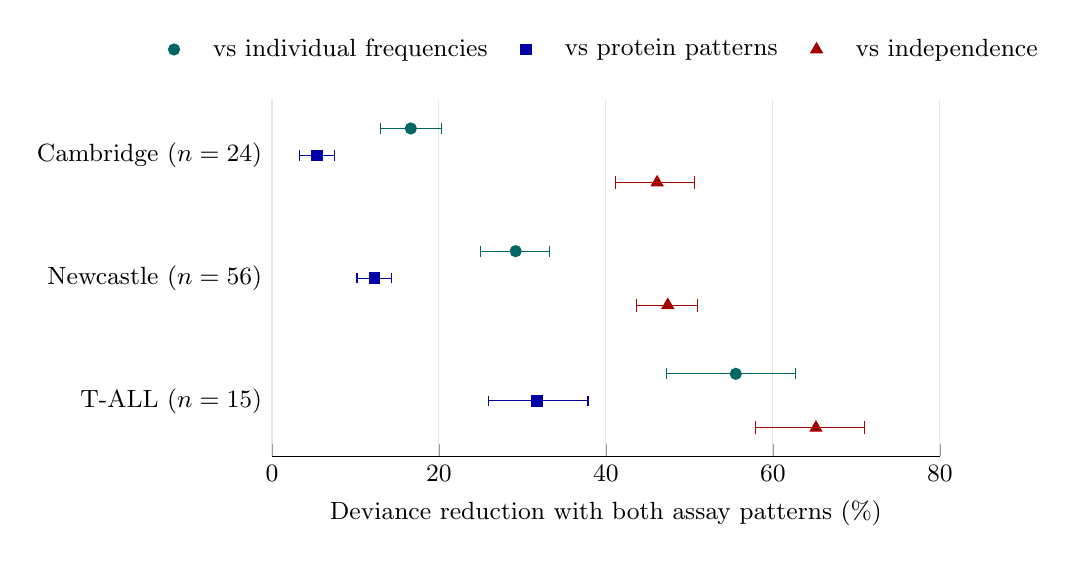
\begin{tikzpicture}
\begin{axis}[
 width=0.83\textwidth,height=6.1cm,
 xmin=0,xmax=80,ymin=0.55,ymax=3.45,
 xtick={0,20,40,60,80},ytick={1,2,3},
 yticklabels={T-ALL ($n=15$),Newcastle ($n=56$),Cambridge ($n=24$)},
 xlabel={Deviance reduction with both assay patterns (\%)},
 axis x line*=bottom,axis y line*=left,y axis line style={draw=none},
 ytick style={draw=none},
 xmajorgrids=true,grid style={black!10},tick style={black!40},
 label style={font=\small},tick label style={font=\small},
 legend style={at={(0.5,1.08)},anchor=south,draw=none,font=\small,
               legend columns=3,column sep=10pt},clip=false]
\addplot[only marks,mark=*,mark size=2pt,color=teal!80!black,
 error bars/.cd,x dir=both,x explicit]
 table[x=x,y=y,x error minus=lo,x error plus=hi,row sep=\\] {
 x y lo hi\\
 16.63216 3.22 3.58227 3.70638\\
 29.19379 2.22 4.19164 4.09033\\
 55.55723 1.22 8.31116 7.11047\\
 };
\addlegendentry{vs individual frequencies}
\addplot[only marks,mark=square*,mark size=1.9pt,color=blue!65!black,
 error bars/.cd,x dir=both,x explicit]
 table[x=x,y=y,x error minus=lo,x error plus=hi,row sep=\\] {
 x y lo hi\\
 5.36225 3 2.03579 2.12418\\
 12.26900 2 2.07730 2.04291\\
 31.75952 1 5.84544 6.10071\\
 };
\addlegendentry{vs protein patterns}
\addplot[only marks,mark=triangle*,mark size=2.4pt,color=red!65!black,
 error bars/.cd,x dir=both,x explicit]
 table[x=x,y=y,x error minus=lo,x error plus=hi,row sep=\\] {
 x y lo hi\\
 46.13638 2.78 4.95309 4.46024\\
 47.40927 1.78 3.79366 3.59373\\
 65.16167 0.78 7.23160 5.83782\\
 };
\addlegendentry{vs independence}
\end{axis}
\end{tikzpicture}

\caption{\textbf{Separate assay patterns improve prediction without scoring-cell summaries.}
Full-pattern reconstruction is compared with three controls at the same
adaptation-derived marker frequencies. Points show relative mean-deviance
reductions; bars are paired recipient-bootstrap 95\% intervals. Each cohort
uses 256 adaptation and 256 scoring cells per person. Protein thresholds,
assay histograms, and marker frequencies use adaptation cells only. The
source interaction is fixed across arms. All nine Bonferroni percentile
intervals have positive lower endpoints; nominal intervals are shown.}
\label{fig:adaptation}
\end{figure*}

\subsection{Within-assay patterns improve dependence prediction}
Conditional on the scoring-cell frequencies, retaining both assay patterns reduced deviance in all three cohorts
(Table~\ref{tab:resolution}). Relative to individual frequencies alone, the
reductions were 36.55\% in Cambridge, 46.85\% in Newcastle, and 72.75\% in T-ALL.
The full-pattern arm improved 23/24, 55/56, and 15/15 recipients, respectively.

\begin{table*}[t]
\caption{Prediction with a fixed source interaction and different assay information.}
\label{tab:resolution}
\centering\small
\begin{tabular*}{\textwidth}{@{\extracolsep\fill}lrrr@{}}
\toprule
Recipient information & Cambridge ($n=24$) & Newcastle ($n=56$) & T-ALL ($n=15$)\\
\midrule
Individual marker frequencies & 0.009606 & 0.015761 & 0.038007\\
RNA patterns and protein frequencies & 0.007982 & 0.012231 & 0.025008\\
RNA frequencies and protein patterns & 0.007106 & 0.010869 & 0.021243\\
Means and covariances (maximum entropy) & 0.006399 & 0.008572 & 0.011553\\
Source pool, matched recipient frequencies & 0.007094 & 0.011927 & 0.029302\\
Cohort pool, matched recipient frequencies & 0.007043 & 0.010446 & 0.021385\\
Both assay-pattern distributions & \textbf{0.006095} & \textbf{0.008377} & \textbf{0.010358}\\
\bottomrule
\end{tabular*}
\par\smallskip\parbox{\textwidth}{\footnotesize Mean donor deviance over all 81 marker pairs;
lower is better. The source interaction, scoring cells, and recipient marker
frequencies were fixed. Pooled controls replaced recipient adaptation profiles
with separate-assay profiles from source donors or other people in the same
cohort, keeping the prior fraction unchanged.}
\end{table*}

Protein patterns gave lower mean loss than RNA patterns in each cohort, but
retaining RNA patterns in addition improved prediction further. Against the
protein-pattern arm, the reductions were 14.23\% in Cambridge (95\% interval,
9.46--19.07\%), 22.92\% in Newcastle (15.71--29.28\%), and 51.24\% in T-ALL
(45.29--57.07\%). All nine Bonferroni percentile intervals had positive lower
endpoints. Retaining RNA patterns therefore improved prediction even when the
full protein-pattern distribution was available.

\subsection{Recipient covariances recover most of the pattern-level gain}
The covariance-preserving replacement retained 91.36\% (paired-bootstrap
95\% interval, 89.09--94.03\%), 97.36\% (96.28--98.38\%), and 95.68\%
(93.42--97.25\%) of the loss reduction from individual frequencies to full
patterns in Cambridge, Newcastle, and T-ALL, respectively. Full patterns improved further
by 4.74\% (95\% interval, 2.81--6.78\%), 2.27\% (1.25--3.37\%), and 10.35\%
(7.59--13.74\%), improving 22/24, 44/56, and 15/15 people. All six contrasts
remained positive under the separate Bonferroni adjustment. Pairwise
within-assay statistics therefore recovered most of the gain, with a smaller
additional benefit from retaining the original patterns.

Recipient-specific covariance also improved on both pooled controls
(Fig.~\ref{fig:resolution}). Against the source pool, deviance fell by
9.80\%, 28.13\%, and 60.57\% in Cambridge, Newcastle, and T-ALL. Against other
recipients in the same cohort, the reductions were 9.15\% (95\% interval,
2.29--15.57\%), 17.94\% (12.58--23.00\%), and 45.97\% (35.24--55.79\%),
with improvements in 15/24, 42/56, and 14/15 people. All six Bonferroni
percentile intervals had positive lower endpoints. Each recipient supplied
256 adaptation cells per assay, compared with 3,072 source cells or
3,584--14,080 cells in the cohort pool. Matching individual frequencies and
using more cells from other people did not recover the recipient-specific gain.

\begin{figure*}[t]
\centering
\definecolor{sourcepool}{HTML}{5D6670}
\definecolor{cohortpool}{HTML}{217D91}
\definecolor{fullpatterns}{HTML}{A64442}
\begin{tikzpicture}
\begin{axis}[
 width=.875\textwidth,height=6.2cm,
 xmin=0,xmax=80,ymin=.55,ymax=3.65,
 xtick={0,20,40,60,80},ytick={1,2,3},
 yticklabels={T-ALL ($n=15$),Newcastle ($n=56$),Cambridge ($n=24$)},
 xlabel={Deviance reduction (\%)},
 axis x line*=bottom,axis y line*=left,
 tick align=outside,y tick style={draw=none},
 xmajorgrids=true,grid style={gray!18},
 axis line style={gray!55},
 tick label style={font=\small},label style={font=\small},
 legend style={draw=none,fill=white,at={(.99,.99)},anchor=north east,
   legend columns=1,font=\small,row sep=3pt},
 legend cell align=left,
 every axis plot/.append style={only marks,mark size=2.4pt,line width=.8pt},
 error bars/x dir=both,error bars/x explicit,
 error bars/error mark options={rotate=90,mark size=3pt,line width=.8pt}
]
\addplot[color=sourcepool,mark=square*] coordinates {
 (9.802959,3.18) += (6.327614,0) -= (6.695547,0)
 (28.127161,2.18) += (5.067868,0) -= (5.241208,0)
 (60.570808,1.18) += (7.427550,0) -= (8.208040,0)};
\addlegendentry{Recipient vs. source pool}
\addplot[color=cohortpool,mark=*] coordinates {
 (9.151773,3) += (6.422499,0) -= (6.860723,0)
 (17.936681,2) += (5.063675,0) -= (5.359103,0)
 (45.974226,1) += (9.818266,0) -= (10.731197,0)};
\addlegendentry{Recipient vs. cohort pool}
\addplot[color=fullpatterns,mark=triangle*] coordinates {
 (4.738083,2.82) += (2.037166,0) -= (1.927312,0)
 (2.274555,1.82) += (1.091061,0) -= (1.025805,0)
 (10.345925,.82) += (3.394911,0) -= (2.756633,0)};
\addlegendentry{Full patterns vs. recipient}
\end{axis}
\end{tikzpicture}

\caption{\textbf{Recipient-specific structure improves dependence transfer.}
Squares and circles compare recipient covariance-preserving reconstruction
with source and other-recipient pools, respectively. Triangles show the further
improvement from full recipient patterns over recipient covariance alone.
Points are relative mean-deviance reductions; lines are paired donor-bootstrap
95\% intervals conditional on the fitted models and pools. All arms use the
same source interaction and recipient marker frequencies. Cambridge and
Newcastle belong to the same study.}
\label{fig:resolution}
\end{figure*}

\subsection{Coexpression prioritizes recipient-specific corrections}
The response score concentrated the recipient-specific gain into relatively
few relationships (Fig.~\ref{fig:relationships}). Its top third accounted for
87.0\%, 90.1\%, and 85.5\% of the net deviance reduction in Cambridge,
Newcastle, and T-ALL, compared with 85.0\%, 60.9\%, and 38.5\% under direct
source-interaction ranking. In Newcastle, the mean gain per selected pair was
0.00506 under the response score and 0.00342 under direct ranking; the paired
difference was 0.00164 (95\% interval, 0.00085--0.00256). In T-ALL the gains
were 0.02523 and 0.01135, a difference of 0.01388 (0.00906--0.01925).
Both contrasts survived the six-comparison adjustment. Cambridge gave similar
gains under the two rankings, 0.00168 and 0.00164 (difference, 0.00004;
$-0.00077$ to 0.00085).

The top-to-bottom-third gain differences were 0.00171 in Cambridge (95\%
interval, 0.00029--0.00330), 0.00498 in Newcastle (0.00318--0.00705), and
0.02426 in T-ALL (0.01648--0.03365). The latter two retained positive
Bonferroni intervals. In T-ALL, the three highest cohort-mean scores were for
CD7 RNA--CD4 protein, CD4 RNA--CD52 protein, and CD7 RNA--CD52 protein;
their mean deviance gains were 0.04513, 0.01245, and 0.04981. The original
study used CD4 and CD7 to distinguish T-cell populations and included CD52 in
a leukemia expression signature \cite{wiggers}. These corrections concern
marker combinations associated with the cohort's cellular heterogeneity.

\begin{figure*}[t]
\centering
\definecolor{cohortpool}{HTML}{217D91}
\definecolor{sourcepool}{HTML}{5D6670}
\begin{tikzpicture}
\begin{groupplot}[
 group style={group size=3 by 1,horizontal sep=.65cm},
 width=.36\textwidth,height=4.7cm,
 xmin=0,xmax=81,ymin=0,ymax=110,
 xtick={0,27,54,81},ytick={0,50,100},
 xlabel={Selected pairs},
 axis x line*=bottom,axis y line*=left,tick align=outside,
 ymajorgrids=true,grid style={gray!18},axis line style={gray!55},
 tick label style={font=\small},label style={font=\small},
 title style={font=\small},
 legend style={draw=none,legend columns=3,font=\small,column sep=8pt},
 every axis plot/.append style={line width=.85pt,mark size=1.8pt}
]
\nextgroupplot[title={Cambridge ($n=24$)},ylabel={Net gain captured (\%)},
 legend to name=relationshiplegend]
\addplot[color=cohortpool,mark=*] coordinates {
 (0,0) (9,80.119066) (18,85.617833) (27,87.020316) (36,98.084592)
 (45,100.426107) (54,101.472095) (63,102.721954) (72,101.154307) (81,100)};
\addlegendentry{Covariance response}
\addplot[color=sourcepool,mark=square*] coordinates {
 (0,0) (9,44.150126) (18,69.710520) (27,85.031480) (36,80.426033)
 (45,80.986286) (54,88.367802) (63,85.716679) (72,92.601559) (81,100)};
\addlegendentry{Direct source strength}
\addplot[color=gray,densely dotted,no marks] coordinates {(0,0) (81,100)};
\addlegendentry{Uniform selection}
\nextgroupplot[title={Newcastle ($n=56$)},yticklabels=\empty]
\addplot[color=cohortpool,mark=*] coordinates {
 (0,0) (9,66.087773) (18,83.699910) (27,90.108397) (36,92.833433)
 (45,96.354103) (54,98.542922) (63,99.582826) (72,99.668898) (81,100)};
\addplot[color=sourcepool,mark=square*] coordinates {
 (0,0) (9,29.400922) (18,46.799828) (27,60.890626) (36,71.959182)
 (45,79.571250) (54,81.847824) (63,85.657623) (72,91.215940) (81,100)};
\addplot[color=gray,densely dotted,no marks] coordinates {(0,0) (81,100)};
\nextgroupplot[title={T-ALL ($n=15$)},yticklabels=\empty]
\addplot[color=cohortpool,mark=*] coordinates {
 (0,0) (9,53.828953) (18,73.403044) (27,85.541946) (36,90.335186)
 (45,94.225120) (54,96.707447) (63,98.146734) (72,99.122589) (81,100)};
\addplot[color=sourcepool,mark=square*] coordinates {
 (0,0) (9,9.524368) (18,25.261325) (27,38.479910) (36,52.136278)
 (45,64.058917) (54,77.324110) (63,83.043000) (72,87.138613) (81,100)};
\addplot[color=gray,densely dotted,no marks] coordinates {(0,0) (81,100)};
\end{groupplot}
\end{tikzpicture}
\par\smallskip\pgfplotslegendfromname{relationshiplegend}

\caption{\textbf{Unpaired coexpression identifies relationships that benefit from correction.}
Pairs are ranked separately within each person. Curves show cumulative
deviance improvement from recipient covariance over the cohort pool, divided
by the net improvement across all 81 pairs. Teal uses the covariance-response
score; gray uses direct source-interaction strength. The dotted line is the
expected fraction under uniform selection. Curves are descriptive cohort
aggregates; donor-bootstrap comparisons at 27 pairs are reported in the text.
Net gain can exceed 100\% when excluded corrections worsen prediction.}
\label{fig:relationships}
\end{figure*}

\subsection{The response ranking persists at fitted strength}
The response coefficient remained closely aligned with exact model discrepancy
throughout the continuation (Additional file 1). At $t=1$, mean
within-recipient Spearman correlations were 0.941 in Cambridge (95\% interval,
0.935--0.948), 0.942 in Newcastle (0.937--0.947), and 0.939 in T-ALL
(0.919--0.954). The response and exact rankings shared 90.3\%, 89.5\%, and
89.1\% of their top 27 queries, respectively. The cohort-aggregate exact
discrepancy at $t=1$ was 40.8\%, 32.1\%, and 28.3\% of the quadratic
approximation.

\section{Discussion}
The resolution at which a relationship is reported need not be the resolution
at which it should be transferred. A binary RNA--protein table depends on the
distribution of finer cellular profiles. Reconstructing those profiles before
aggregation allowed one source interaction to predict different recipient
associations using measurements made separately within each assay. The
adaptation-only analysis establishes this advantage without supplying
scoring-cell summaries. The conditional analysis then separates the
contribution of coexpression from marginal-frequency estimation error.

The pooled controls distinguish recipient-specific coexpression from generic
population structure: more observations from other people did not replace
the recipient's own assay patterns. Equation~\eqref{eq:response} explains how
within-assay covariances alter the association induced by a fixed source
interaction. It also explains why ranking direct source coefficients can miss
relationships that change in a recipient. The response score uses the
covariances around each query to identify these relationships, improving
prioritization in two cohorts. At the other extreme, the coarsening bound
describes the range of associations left unresolved when those measurements
are unavailable. Together, these results connect the detail retained in
separate assays to both the limits of prediction and the choice of queries.

\section{Limitations}
The analyses are retrospective evaluations of previously examined recipients
from two studies, not new confirmation. The adaptation-only test changes the
protein-state definition as well as the information boundary; its effect sizes
cannot be subtracted from the conditional results to measure information leakage.
Intervals condition on the source fit and fitted pools, omitting their
estimation uncertainty, dependence between overlapping cohort pools, and the
adaptive research history.

The panel contains nine RNA and nine protein markers. The conditional analysis
uses donor-wide protein ranks and individual scoring-cell marker frequencies;
the adaptation-only analysis uses neither. Two Stephenson recipients have almost no counts across
the protein panel and were retained. The task is fixed-margin dependence
prediction from separately measured assays, not missing-modality imputation
without target assay observations. The
results do not isolate within-cell-type regulation or establish molecular
binding, causal effects, or clinical utility.

The identified interval assumes a known transferable interaction, finite
assay supports, and exact recipient summaries. Its all-marker endpoints require
global optimization over the corresponding marginal polytopes; only the
two-frequency case has the closed form reported here. The examples establish
ambiguity, not its biological magnitude. Query-wise minimax predictions need
not form a coherent multivariate law. Interaction drift, sampling error, and
coarsening ambiguity remain distinct.

We tested one maximum-entropy replacement, which preserves fitted means and
covariances but can induce higher-order correlations. The retained
gain is descriptive, not causal mediation. The exact response identity holds
at finite strength, but the quadratic coefficient overestimated the magnitude
of model discrepancy at $t=1$. Its query score predicts model discrepancy, not
error against an arbitrary biological population. The query-ranking advantage over direct source strength
was unresolved in Cambridge. Prioritization requires the full measured panel
and does not establish savings from measuring fewer markers. Sorting and cell
mixtures can contribute to the observed coexpression.

Reconstruction, noncollapsibility, and minimax KL prediction have established
foundations. The theory concerns the resolution-dependent identified set;
the experiments establish an information advantage, not a superior interaction
learner. The earlier matched CHAMPOLLION-objective comparison did not establish
superiority and remains documented with the historical benchmark.

\section{Conclusions}
Within-assay cellular patterns improved cross-cohort RNA--protein prediction
with the source interaction held fixed, including prediction on untouched cells
without their marginal summaries. In the conditional analysis, recipient-specific
covariances retained most of the pattern-level gain and outperformed source and cohort
pools matched to the same marker frequencies. Full patterns improved further
in each cohort. Separately measured recipient coexpression can therefore
support molecular predictions that individual frequencies and cohort averages
do not recover.


\section*{Abbreviations}
CITE-seq: cellular indexing of transcriptomes and epitopes by sequencing;
KL: Kullback--Leibler; RNA: ribonucleic acid;
T-ALL: T-cell acute lymphoblastic leukemia.

\section*{Declarations}

\subsection*{Ethics approval and consent to participate}
This study used only public, de-identified data and involved no new participants, specimens, interventions, or identifiable records; the original studies report their ethics approvals and consent procedures.

\subsection*{Consent for publication}
Not applicable.

\subsection*{Availability of data and materials}
Source data are available under E-MTAB-10026 (Stephenson CITE-seq) and
GSE248287 (T-ALL). The original benchmark's analysis plans,
software, and study records are available in the v2.0.4 release
\cite{benchmark2026}. The accompanying analysis artifact contains derived
assay distributions, reconstruction code, predictions, and recipient-level
losses for the subsequent resolution analyses, together with executable
checks of the reported comparisons. Additional file 1 specifies the protocols.
Raw matrices are not redistributed.

\subsection*{Competing interests}
Competing-interest information is withheld in the blinded manuscript.

\subsection*{Funding}
Funding information is withheld in the blinded manuscript.

\subsection*{Authors' contributions}
Author names and contribution statements are withheld in the blinded manuscript.

\subsection*{Acknowledgements}
OpenAI Codex assisted with code development, literature retrieval, manuscript
editing, and \LaTeX{} preparation.

\subsection*{Additional file}
Additional file 1 (PDF). \emph{Mathematical results and analysis protocols}.
Identified-set and response proofs, adaptation-only and conditional protocols,
cohort-level comparisons, and computational verification.

\ifdefined\ReaderVersion\else
  \setlength{\bibsep}{3pt}
\fi
\begingroup
\ifdefined\ReaderVersion\balance\fi
\renewcommand{\bibfont}{\normalfont\small}
\raggedright
\interlinepenalty=10000
\bibliography{references}
\endgroup

\end{document}
